\documentclass[11pt,a4paper,titlepage]{article}
\usepackage{times}
\usepackage{graphics}
\usepackage{dmacros}
\setlength{\oddsidemargin}{0cm}
\setlength{\evensidemargin}{0cm}
\setlength{\marginparwidth}{0cm}
\setlength{\marginparsep}{0cm}
\setlength{\topmargin}{0cm}
\setlength{\headheight}{0cm}
\setlength{\headsep}{0cm}
\setlength{\textheight}{24cm}
\setlength{\textwidth}{16cm}
\setlength{\footskip}{1.5cm}
\renewcommand{\baselinestretch}{1.1}

\tolerance=2600
\hbadness=2000
\hyphenpenalty=1000
\doublehyphendemerits=1000000

\skip\footins = 18pt plus 1fil
\renewcommand{\footnoterule}{\kern -6pt \hrule width 2in \kern 5.6pt}
\renewcommand{\thefootnote}{$\ast$} 

\hyphenation{seismo-graphic}

\title{SeisComP 2.1 Manual}
\author{Andres Heinloo, GFZ Potsdam \\ Chad Trabant, KNMI }
\date{June 28, 2004}

\begin{document}
\maketitle

\setcounter{page}{2}

%%%%%%%%%%%%%%%%%%%%%%%%%% Table of Contents %%%%%%%%%%%%%%%%%%%%%%%%%%%%%%


\tableofcontents

\clearpage

%%%%%%%%%%%%%%%%%%%%%%%%%%%%%%%%%%%%%%%%%%%%%%%%%%%%%%%%%%%%%%%%%%%%%%%%%%%

\section{Introduction}

The Seismological Communication Processor (SeisComP) is a new concept for a
networked seismographic system, originally developed for the GEOFON network
and further extended within the MEREDIAN project under the lead of
GEOFON/GFZ Potsdam and ORFEUS. SeisComP resources can be found at the
following locations:

\begin{table}[h!]
\centering
\begin{tabular}{ll}
SeisComP homepage at GFZ      & http://www.gfz-potsdam.de/geofon/seiscomp/ \\
SeisComP homepage at ORFEUS   & http://orfeus.knmi.nl/meredian/seiscomp/   \\
SeisComP mailing list archive & http//geofon.gfz-potsdam.de/seiscomp-l/    \\
\end{tabular}
\end{table}

The task of SeisComP is six-fold:
\begin{itemize}
\item data acquisition
\item data recording
\item monitoring and controlling
\item real-time communication
\item user access
\item automatic (N)RT data processing (quality control, event detection and
location)\footnote{Not covered by this manual}
\end{itemize}

The primary software components have been released as a software
package called simply SeisComP. The core of the software package is
the SeedLink data acquisition system. SeedLink clients connect to the
server using a robust TCP/IP application level protocol (SeedLink
protocol). The following clients are included in the package:
\begin{description}
\item[slarchive] saves data to the disk in Mini-SEED format, using
either the SDS (SeisComP Data Structure), BUD (Buffer of Uniform Data)
or a user-defined directory structure.

\item[slqplot] is used to plot traces in real time, either in an
X-Window or by creating image files.

\item[slinktool] is used mainly for testing a SeedLink server and to
get information about the available stations, time spans of streams,
gaps, etc. See section~\ref{slinktool}.
\end{description}

The package also includes the \verb+libslink+ software library with
its own documentation, which can be used by C programmers to create
their own clients. For backwards compatibility a version of Comserv
running in parallel with SeedLink is included in the package as well.

The data source for a SeedLink server can be anything which is
supported by a SeedLink ``plugin''. Data supplied by a plugin can be
in the form of 512-byte Mini-SEED packets or just raw integer samples
with associated timing and naming information. In the latter case, the
SeedLink server uses an integrated, highly configurable Stream
Processor to create the desired datastreams and assemble Mini-SEED
packets. The following plugins are included in the package:
\begin{description}
\item[serial\_plugin] supports Earth Data PS2400/PS6-24 (3 and 6 channels),
Guralp DM24, Geotech DR-24 digitizers (HLCP protocol), and Prema DMM
5017 Digital Multimeter (experimental).

\item[m24-plug] supports Lennartz M24 (contributed by Lennartz
Electronic GmbH).

\item[chain\_plugin] is used to connect to remote SeedLink systems.

\item[sock\_plugin] is used to connect to remote LISS systems.

\item[naqs\_plugin] is used to connect to remote Nanometrics NAQS
systems.

\item[fs\_plugin] is used to feed data from files (Titan, Seisan or
Mini-SEED format) into SeedLink (near-real time).

\item[comserv\_plugin] is used to feed data from Comserv into
SeedLink. This allows acquisition from older generation Quanterra
digitizers (Q380/Q680, Q4120, Q720, etc.).

\item[q330\_plugin] supports the Quanterra Q330 (based on Quanterra's
Mountainair software).

\item[reftek\_plugin] acquires data from RefTek daemon (RTPD).

\item[ewexport\_plugin] collects data from an Earthworm export\_* process.

\item[scream\_plugin] collects data from Guralp's SCREAM! server.
\end{description}

More plugins (Kinemetrics K2, Lennartz MARS-88, Lennartz PCM 5800, Visitec,
Geoscope CCU, MK6) have been contributed, but not (yet) included in the
package. The included C language plugin interface is described in
section~\ref{plugins}.

The clients \verb+slink2orb+ and \verb+slink2ew+ can be used to import
data from SeedLink directly into Antelope and EarthWorm respectively.
\verb+orb_plugin+ can be used to import data from an Antelope ORB into
SeedLink. In order to compile these modules, the development
environment of a corresponding system is needed. These packages can be
downloaded from ftp://orfeus.knmi.nl/pub/software/seiscomp/.

An overview of SeedLink connectivity is shown on figure~\ref{overview}.

In order to simplify the installation procedure SeisComP configuration
files can be created automatically, using "key files" to fill in
templates.  However, for advanced configuration, it is necessary to
modify the generated configuration files or templates by hand.

\begin{figure}[p!]
\centering
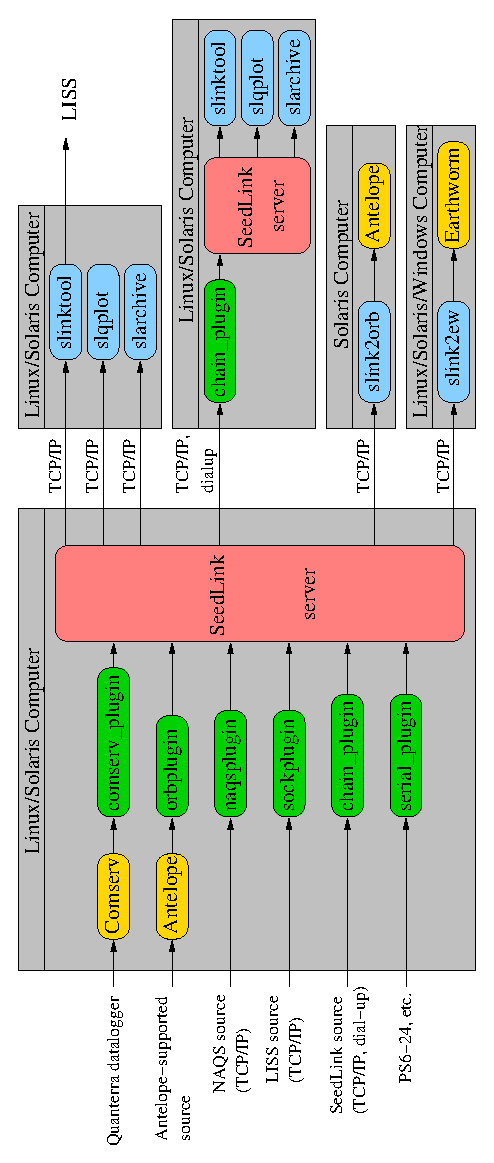
\includegraphics{overview.eps}
\caption{Overview of SeedLink connectivity} \label{overview}
\end{figure}


\section{Installation Procedure}

\begin{enumerate}
\item Create a user account that uses the "bash" shell (the preferred
user name is "sysop" with home directory "/home/sysop").

\item If you want to have an interactive (telnet-based) data request
manager (DRM), create a second user account that uses the "tcsh"
shell, having a different user ID, but the same group ID and working
directory as "sysop".  Then add "umask 002" to ~/.bashrc. (\textbf{DRM
is currently not maintained and may not work correctly!})

\item Unpack the SeisComP binary distribution in "/home/sysop" or
whatever directory you chose in step 1. This creates directories
"/home/sysop/\{bin,doc,man,templates\}".

\item Create a "key file", using the \verb+bin/make_key+ utility. If
you want to add more stations, run \verb+bin/make_key+ again. See
section~\ref{makekey}.

\item Run \verb+bin/make_conf+ to create the configuration files for all
stations from templates.

\item Log in as root and run \verb+bin/make_root+, which does the
following:
\begin{itemize}
\item Sets permissions (rw,rw,rw) on serial ports used by the digitizer.

\item Sets permissions (rwx,rx,rx) on sysop and DRM home directories.

\item Sets permissions (rwx,rwx,rwx) on /var/spool/uucp (required by Kermit).

\item Links config/stations.ini and config/network.ini to /etc (required by
Comserv).

\item Links bin/leapseconds to /usr/local/lib.

\item Links data to /nrt (required by DRM).

\item Sets suid bit on bin/m24-plug (so it can use the real-time
scheduler) if Lennartz M24 digitizer is used.
\end{itemize}

If none of the above is needed (or done manually), then running
\verb+bin/make_root+ is not necessary.

\item Log in as "sysop" or whatever login name you chose in step 1 and
you will be in the SOM menu (Station Operation Manager). See
section~\ref{som}.
\end{enumerate}

For advanced configuration it might be necessary to modify the generated
configuration files by hand. It is also possible to edit the templates
files such that subsequent runs of \verb+bin/make_conf+ produce the desired
configuration. \textbf{\texttt{make\_conf} removes the content of
``config'' directory, so any manual changes in config files will be lost!}
Therefore it is recommended to keep a copy of modified config files in
another directory.

\subsection{Station and Stream Identifiers}

Any station is uniquely identified by a network code and station
code. In fact the station code alone uniquely identifies the site, but
if the station is jointly operated by several networks, the data of
the same station may be available with different network codes.

In some rare situations it may be desired to have more than one
station with the same station code, but different network codes
configured on the same SeisComP system, so we cannot simply use
station code as a station identifier in SeisComP. However, always
using a combination of network code and station code is clumsy and
besides not supported by Comserv.

For this reason any station in SeisComP is also assigned a ``station
ID''.  Normally a ``station ID'' is the same as the associated station
code, but if the station code is already in use a different station ID
is allocated. Station IDs are needed for working with the SOM and
\verb+seiscomp_ctrl+ control script. SeedLink uses Station IDs when
communicating with plugins, so it is important that the Station IDs
SeedLink is expecting match the IDs plugins are using. Station IDs are
strictly local to the SeisComP system and never seen by remote
SeedLink clients.

Any datastream of a station is uniquely identified by SEED channel
code (\textit{seedname}), location code and type. Channel codes and
location codes exist in the header of Mini-SEED records, while type is
assigned to each record depending on the blockettes it contains.

In order to request data from a SeedLink server it is necessary to
know the IP address (or hostname) and TCP port of the server as well
as the codes of desired stations.  The data content of a server
(available stations and streams) can be checked with \verb+slinktool+.


\subsection{Using the \texttt{make\_key} Utility}\label{makekey}

The \verb+make_key+ utility asks the user a series of questions. Some
questions have default answers in square brackets. To choose a default
answer, enter an empty string. The questions are explained below:
\begin{interface}
\item Organization [GEOFON DC]:

Organization ID, shown with \verb+slinktool -I+; arbitrary string.

\item Default network code [GE]:

Network code, used when a network code is omitted by a client in
STATION request. Should be set to the network code of the majority of
configured stations. Can be 1 or 2 characters long, uppercase.

\item Operator login name [sysop]:

Login name of the SeisComP account, normally "sysop".

\item Install SeedLink [yes]:

Answer "yes" to install a local SeedLink server; "no" if you do not
have local digitizers and want all the clients to connect directly to
remote servers (this will multiply the required bandwidth by the
number of clients used). "Yes" recommended.

\item Install Digiserv (required for triggering) [no]:

Answer "yes" to install a second local SeedLink server as a primary
server. This makes it possible to use certain advanced features like
resampling and triggering. "No" recommended. (See also
section~\ref{schemes}.)

\item Install Data Request Manager (DRM) [no]:

Answer "yes" to install the telnet-based DRM (second account needed). Not
recommended.

\item Maintain datalog compatibility links in /home/sysop/data [no]:

Answer "yes" if you want to use \verb+slarchive+ (recommended), but also
install cron job that creates symbolic links under /home/sysop/data
(updated every night), following the conventions of \verb+datalog+
(obsolete). Not recommended, unless needed for backwards compatibility.

\item Station code:

Name of your local station or the station you want to request from a
remote server; up to 5 characters, uppercase.

\item Station description [GEOFON_Station]:

Station description, shown with \verb+slinktool -L+; arbitrary string.

\item Network code [GE]:

Network code of the station; 1 or 2 characters, uppercase.

\item Type of data source [0]:

If connecting to a remote SeisComP, enter 0 (SeedLink), otherwise
choose the appropriate type of the digitizer or data acquisition
system. This option determines which plugin is used and some other
settings.

If the data source is based on TCP/IP, you are now asked about the IP
address and port. In case of a local data source, the path to device file
is asked.

\item Stream processing scheme [stream_50]:

Unless the source data is already in Mini-SEED format, the name of stream
processing scheme is asked. That is required in order to create Mini-SEED
records from raw streams. The stream processing scheme selected must be
defined in streams.xml and match the configuration of input channels
(see also section~\ref{streamsxml}).

\item Data port [/dev/data]:

The default setting (/dev/data) works if you have created such a
symbolic link, pointing to the real device file. The usual settings
are "/dev/ttyS0" for COM1, "/dev/ttyS1" for COM2 and "/dev/ttyUSB0"
for a USB-serial adapter.

\item IP address or hostname [192.10.10.10]:

Address of the remote server.

\item TCP port [18000]:

Remote TCP port, normally 18000 if the remote server is SeedLink.

\item SeedLink mode [0]:

Here you can choose real-time or dial-up mode. Using dial-up mode only
makes sense (apart from testing) if you have a dial-up (modem, ISDN,
e.g., not flat-rate Internet) connection to the server. Configuring
dial-up mode is explained further in section~\ref{dialup}.

\item Stream selectors:

If you want to get all available data leave it empty. Otherwise enter the
selectors (uppercase, separated by space), e.g. \verb+BH?.D+. For more
information, refer to the \verb+slinktool+ manpage.

\item Triggered HH streams [no]:

Iy you answered ``yes'' to ``Install Digiserv'' earlier, then here is a
possibility to activate the event detector to trigger HH streams. In this
case it would be probably necessary to fine-tune the trigger parameters in
trigger.ini. The detector module is implemented in Python, so Python must
be installed and functional. In order to trigger other streams than HH*,
chain.xml and trigger.ini must be edited.

\item Default disksize in MB per stream [50]:

Data files created by \verb+datalog+ will be deleted by a cron job to keep
the amount of data per stream under the given limit. Now obsolete.

\item Maximum number of days to keep datafiles [50]:

Data files created by \verb+slarchive+ will be deleted by a cron job when
older than this many days.

\item Install Comserv [no]:

This question is only asked if the type of data source is not
"Quanterra".  In this case using Comserv is optional and not
recommended. If you answer "yes" here then Comserv will run as a
client of SeedLink and you will be asked a couple of comserv specific
questions.

\item Comserv segment ID [9600]:

The ID of station's shared memory segment. Arbitrary number, but must be
unique for each station configured.

\item Install datalog [no]:

Datalog is an old version of \verb+slarchive+ that runs as a client to
Comserv.  Now obsolete.

\item Install slarchive [yes]:

Anwer "yes" if you want to keep a local data archive (e.g. not merely
running the machine as a SeedLink server). Using \verb+slarchive+ is
in any case recommended for backup purposes. The data archive will be
located in "archive" subdirectory, structured according to the SDS
specification (see also section~\ref{sds}). For more information about
slarchive consult the manpage.

\item slqplot filter [WWSSSP]:

IIR filter used by \verb+slqplot+. WWSSSP (WWSSN short period seismograph
simulation) recommended.

\item slqplot magnification factor [50000]:

Normally between 5000 (noisy station) and 50000 (quiet station). Also
depends on the gain of the seismometer and digitizer.

\item Install permanent slqplot daemon for GIF-file creation [no]:

Answer "yes" if you want to have plots in GIF format (one per day +
"active" plot updated every 10 minutes by a cron job). In this case you
will be asked the following two questions:

\item GIF-file size [1024x780]:

Default recommended.

\item Number of days to keep old GIF-files [30]:

GIF files will be deleted by a cron job when older than this many of
days.

\end{interface}


\subsection{Configuring Dial-up Mode}\label{dialup}

Dial-up mode is useful if data is transferred over communication lines
where the costs are related to the connection time and the operator
thus wishes to minimize the connection time.  Using dial-up mode
connections will not be kept permanently open but rather opened
periodically for a short time to download all data collected since the
last connection.

A prerequisite of using dial-up mode is that both the server and
client machine are properly configured for dial-up connections using
the operating system facilities (pppd, mgetty, etc.). As far as
SeisComP is concerned only the client side needs special configuration
because the client initiates the connection and selects dial-up mode.

If you choose dial-up mode \verb+make_key+ will ask the following
questions:
\begin{interface}
\item Dial-up schedule [0,30 * * * *]:

This is the schedule, in crontab format, which specifies when the
connection is initiated. The default is every full and half hour; for
other options refer to the crontab manpage. The connection is
initiated by \verb+chain_plugin+ (see also section~\ref{schemes});
crond is not involved.

\item Uptime [900]:

The \textbf{maximum} time to keep the connection open. In dial-up mode
the connection is closed as soon as all available data is transmitted
(in fact that is the only difference between real-time and dial-up
mode as far as SeedLink is concerned).
\end{interface}

More advanced options can be found in chain.xml (see
section~\ref{chainxml}).

\subsection{Uninstalling Stations}

In order to remove a station from the system the respective keyfile
under ``key'' subdirectory can simply be removed. After running
\verb+make_conf+, the station is no longer configured. 
\verb+make_conf+ should be, however, used with caution as it
overwrites all configuration files and any manual changes will be lost.


\section{Station Operation Manager}\label{som}

After the installation procedure is finished and you log in as ``sysop''
(or whatever login name you chose), the Station Operation Manager (SOM) is
started. It asks for your initials (these are logged in logs/initials.log)
and default station ID (if more than one stations are defined). After
that, the main menu is displayed:

\begin{verbatim}
    SOM Main Menu
    
    a - Control data aquisition
    p - Control monitor plots
    o - Escape to Linux shell
    w - Switch to other station

    q - quit
    
Command --->
\end{verbatim}

Following options are provided:
\begin{description}
\item[a - Control data acquisition] takes you to the Acquisition Control Menu:

\begin{description}
\item[s - Start data acquisition] starts SeedLink (if configured) and all
configured local clients of all stations. Also installs the SeisComP crontab.

\item[k - Stop data acquisition] stops SeedLink (if configured) and all
configured local clients of all stations. Removes the SeisComP crontab.

\item[b - Start current station] starts SeedLink (if configured) and all
configured local clients of the default station.

\item[t - Terminate current station] stops all configured local
clients of the default station (SeedLink is not stopped).
\end{description}

\item[p - Control monitor plots] takes you to the Plot Menu:

\begin{description}
\item[x - Start default plot in X-window] starts real-time plotting of
the default station in an X-window. Plot configuration can be changed
in config/slqplot\_\textit{station} (see also section~\ref{slqplotini}).

\item[X - Abort default X-window plot] stops the real-time plotting of
the default station.

\item[h - Change display host] changes the DISPLAY environment variable.
Set it to \textit{hostname}:0.0.
\end{description}

\item[o - Escape to Linux shell] takes you to the user login shell, where
command-line utilities can be used (see also section~\ref{commandline}).

\item[w - Switch to other station] changes the default station.
\end{description}


\section{Command-line Utilities}\label{commandline}

\subsection{\texttt{seiscomp\_ctrl}}

Instead of using the ``b'' and ``t'' options in the Acquisition Control Menu,
you can start and stop all local SeedLink clients of a single station with
\verb+seiscomp_ctrl+. The syntax is \\ \verb+seiscomp_ctrl+
\textit{\{}\texttt{start}$|$\texttt{stop}$|$\texttt{check}\textit{\} station
station...}, \\
where \textit{station} is a station ID.

It is harmless to use the ``start'' option when local clients are already
running. SeisComP uses lockfiles to ensure that superfluous program
instances are not started.

The third option, ``check'', only starts the station if it is not previously
stopped by \verb+seiscomp_ctrl+. It is normally called from crontab.

When omitting the station names, the full start or stop is performed
for all stations (including SeedLink). However, \verb+seiscomp_ctrl+
does not change the SeisComP crontab (unlike ``s'' and ``k'' options
in the Acquisition Control Menu), so the crontab must be installed or
removed manually.


\subsection{\texttt{slinktool}}\label{slinktool}

The \verb+slinktool+ utility can be used to check the status of a SeedLink
server as well as request data. Here are few examples:
\begin{interface}
\item slinktool -I localhost:18000

Shows general info about the server, including software version.

\item slinktool -L localhost:18000

Shows the list of stations available from the server.

\item slinktool -Q localhost:18000

Shows the timespan of data streams in SeedLink's ring buffer.

\item slinktool -G localhost:18000

Shows the data gaps (missing data) in SeedLink's ring buffer.

\item slinktool -C localhost:18000

Shows the status of connections.

\item slinktool -i all localhost:18000

Sends a generic query and returns the XML document. DTD of the document is
given in section~\ref{infodtd}.

\item slinktool -S 'GE_APE:BHZ.D' -o data.mseed localhost:18000

Requests stream BHZ.D of station APE (network GE) and saves the result to
file data.mseed (real-time).

\item slinktool -tw 2002,10,11,06,00,00:2002,10,11,06,10,00 -S
'GE_CART:BHZ.D' -o data.mseed localhost:18000

Requests time window and saves the result in data.mseed.
\end{interface}

Note that the maintainer of the SeedLink server may restrict the
information available. For more information about slinktool, have a
look at the manpage.


\subsection{SeedStuff}

SeedStuff is a collection of utilities that work with SEED data files
(e.g. files created by \verb+slarchive+). Some of these utilities are
included in SeisComP. Here are few examples:
\begin{interface}
\item check_file data.mseed -B 512

Shows the content of file data.mseed (time span, gaps, etc.).

\item check_seed data.mseed -B 512 -a

Similar but with more verbose output (only non-multiplexed files).

\item extr_file data.mseed -B 512

Demultiplexes a multiplexed file.

\item extr_file data.mseed -B 512 -b 021011_060000 -e 021011_061000

Extracts time window from file.

\item extr_file data.mseed -B 512 -f a

Converts file into ASCII format.
\end{interface}

The utilities will show help information when called without arguments.


\section{Configuration Schemes}\label{schemes}

If you answer ``no'' to the question ``Install SeedLink'' when using
\verb+make_key+, no local SeedLink server will be configured, and all
clients connect directly to remote server(s). Because each client has its
own connection to the server, the same data may be be transferred over the
Internet many times. A permanent Internet connection is required (no
dial-up). This kind of setup is shown on figure~\ref{scheme1}.

\begin{figure}[p!]
\centering
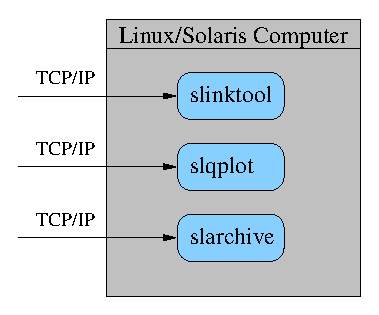
\includegraphics{scheme1.eps}
\caption{SeisComP setup without local SeedLink server} \label{scheme1}
\end{figure}

In most cases, however, a local SeedLink server is used as shown in
figure~\ref{scheme2}. In this case only a single connection (via
chain\_plugin) is established to each of the servers, minimizing the
consumed Internet bandwidth.

\begin{figure}[p!]
\centering
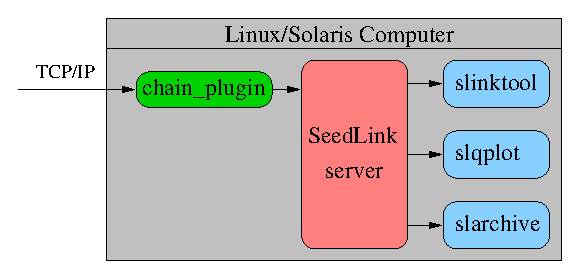
\includegraphics{scheme2.eps}
\caption{SeisComP setup with local SeedLink server} \label{scheme2}
\end{figure}

In some special cases it is desired to run two SeedLink servers as shown
on figure~\ref{scheme3}. This will be configured if you answer ``yes'' to
the question ``Install Digiserv'' of \verb+make_key+. (The primary SeedLink
server is called ``Digiserv'').

\begin{figure}[p!]
\centering
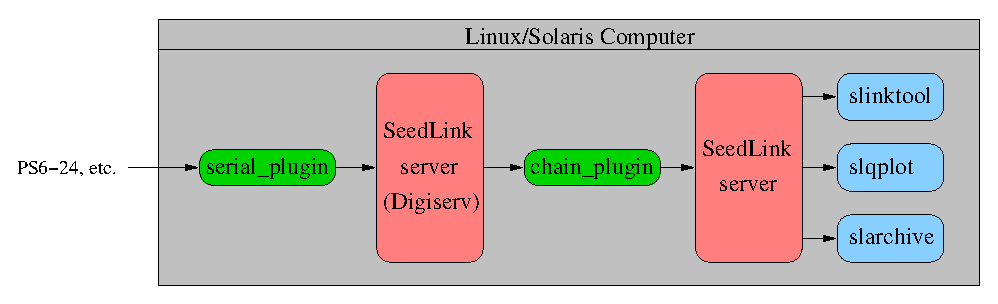
\includegraphics{scheme3.eps}
\caption{SeisComP setup with local SeedLink and Digiserv} \label{scheme3}
\end{figure}


\section{SeisComP Configuration Files}

After running the \verb+make_conf+ utility the following files will be
created in the ``config'' subdirectory (\textit{station} denotes
station ID):
\begin{description}
\item[rc\_\textit{station}] some parameters used by SOM and other scripts.
SOM and \verb+seiscomp_ctrl+ obtain the station list based on these files.

\item[clients\_\textit{station}] client list of \textit{station}, used by
\verb+seiscomp_ctrl+.

\item[slqplot\_\textit{station}] slqplot configuration for
\textit{station}. See also section~\ref{slqplotini}.

\item[station\_\textit{station}] main configuration file of Comserv
(obsolete). Needs a symbolic link from data/\textit{station}\slash
station.ini. See Comserv documentation.

\item[stations.ini] additional configuration file for Comserv (obsolete).
Needs a symbolic link from /etc\slash stations.ini, created by
\verb+make_root+. See Comserv documentation.

\item[network.ini] configuration file for Netmon (obsolete). Needs a
symbolic link from /etc/network.ini, created by \verb+make_root+. See
Comserv documentation.

\item[plugins.ini] configuration file for SeedLink plugins. Used by
\verb+serial_plugin+, \verb+fs_plugin+ and \verb+comserv_plugin+.

\item[seedlink.ini] main configuration file for SeedLink. See also
section~\ref{seedlinkini}.

\item[filters.fir] coefficients of SeedLink's decimating FIR
filters. If a filter's name ends with ``M'', it is a minimum-phase
filter -- causal filter with minimized (non-constant) phase delay;
since the filter is non-symmetric all coefficients must be
given. Otherwise the filter is a zero-phase filter -- non-causal filter
with zero phase delay; in this case the filter is symmetric and so
only half of the coefficients must be given (it is not possible to use
a zero-phase filter with an odd number of coefficients).

\textbf{Important note:} The coefficients for non-symmetric (minimum-phase)
FIR filters in the filters.fir file are stored in reverse order.  It is
important to reverse the order of coefficients if the operator adds a new
minimum-phase filter or uses the included minimum-phase filters for another
application.  The coefficients for symmetric (zero-phase) FIR filters are
not stored in reverse order.  As a sanity check for symmetric filters the
largest coefficient is always in the middle of the symmetry.

\item[streams.xml] SeedLink stream configuration file for the internal
Stream Processor, referenced from seedlink.ini. See also
section~\ref{streamsxml}.

\item[chain*.xml] configuration file for \verb+chain_plugin+. If one chain
is used (no Digiserv), the file is called chain.xml. Otherwise there will
be two files: chain\_digiserv.xml and chain\_seedlink.xml. See also
section~\ref{chainxml}.

\end{description}

DTDs corresponding to the XML configuration files are included in the
SeisComP package and also shown in appendix~\ref{dtds}. An XML file can be
checked against it's DTD (``validated'') with the \verb+xmllint+ utility
like this:

\begin{verbatim}
xmllint --noout --noblanks --dtdvalid streams.dtd streams.xml
\end{verbatim}

\verb+xmllint+ is a part of ``libxml2'' package that can be downloaded from
http://www.xmlsoft.org/.

INI files have a somewhat obscure syntax. They contain zero or more
\emph{sections}, each beginning with a section name in square braces
which should appear on a line of its own.  Section name cannot contain
spaces and square braces, but it can be optionally surrounded by
spaces. Each section consists of zero or more
entries -- \emph{definitions} and \emph{assignments}. A definition
consists of a \emph{keyword} and a \emph{name} separated by spaces
(e.g. ``station EDD'').  An assignment consists of a \emph{parameter}
and a \emph{value} separated by the ``='' sign and optionally
surrounded by spaces (e.g. ``network = GE'').

The set of assignments that immediately follow a definition is in the scope
of that definition. Assignments in the beginning of a section are
``global'' -- they are used to set some generic parameters and provide
default values (e.g.  ``network = GE'' in the beginning of the section sets
the default network that can be overridden in the scope of a station
definition).

Parameters and keywords are case insensitive and must not contain
symbols ``='', ``['', ``]'' or spaces. Names must not contain ``=''
signs or spaces. Values must not contain ``='' signs or spaces, unless
enclosed in double quotes. Double quotes that are part of the value
itself must be preceded by ``$\backslash$''. Each assignment must be
complete on a single line, but several assignments can appear on one
line, separated by spaces. Any line beginning with a ``\#'' or ``*''
character is regarded as a comment and ignored.

\newcommand{\dfl}[1]{[#1]}

\subsection{slqplot.ini}\label{slqplotini}

Usually there is one slqplot configuration file per station called
slqplot\_\textit{station}. The file may contain several sections, but only
one, either having the same name as the executable or specified with the
``-c'' commandline option, is used. A section in qplot.ini has the
following structure (default values, if applicable, are shown in square
brackets\footnote{It is generally not recommended to rely on default
values, because they may change in future versions.}):
\begin{description}
\item[parameter ``tracelen'' \dfl{180}] length of a trace in minutes.

\item[parameter ``traces'' \dfl{8}] number of traces (per channel) on
screen.

\item[parameter ``scroll\_step'' \dfl{1}] how many traces to scroll when
end of page is reached.

\item[parameter ``complete\_pages'' \dfl{no}] if ``yes'' wait until all
channels have reached the end of page. If ``no'' scroll as soon as the
first channel reaches the end of page.

\item[parameter ``coloured\_traces'' \dfl{no}] if ``yes'' use different
colors for subsequent traces. Colors are not supported by all output
devices; in textronix format special control sequences are used which are
only supported by the \verb+tek2gif+ program.

\item[parameter ``desc1''] station description on top of the screen, line~1.

\item[parameter ``desc2''] station description on top of the screen, line~2.

\item[keyword ``channel'' (\textit{seedname})] Adds one channel to the
plot. E.g., ``channel BHZ''.

\begin{description}
\item[parameter ``location''] select channel with a given location code.

\item[parameter ``mag'' \dfl{1000}] magnification which is defined such
that if $mag = 1$ 24-bit fullscale traces touch each other but do not
overlap. Usual values are between 5000 and 50000.

\item[parameter ``filter''] name of IIR filter used. Filters are defined in
a file selected with the ``-F'' command-line parameter of slqplot.

\item[parameter ``fmag'' \dfl{100}] additional magnification used when
filtering.
\end{description}

\item[keyword ``plot'' (\textit{format})] adds one output display.
Supported formats are ``x'', ``ps'', ``hpgl'', ``tek'' and ``meta''. E.g.,
``plot tek''.

\begin{description}
\item[parameter ``display''] name of X display, overrides the DISPLAY
environment variable. (Applicable to ``x'' format.)

\item[parameter ``term''] terminal type, overrides the TERM environment
variable. Applicable to ``tek'' format.

\item[parameter ``file''] output file. If the value starts with a ``$|$''
output is sent to a pipe. First occurrence of ``*'' is replaced with a
timestamp. Applicable to all formats except ``x''.

\item[parameter ``fg'' \dfl{black}] foreground color.

\item[parameter ``bg'' \dfl{white}] background color.

\item[parameter ``size'' \dfl{1024x682}] size of display in pixels.
(Applicable to ``x'' format.)

\item[parameter ``paper'' \dfl{a4}] paper size. Applicable to ``ps'' and
``hpgl'' formats.

\item[parameter ``orientation'' \dfl{landscape}] ``portrait'' or
``landscape''. Applicable to ``ps'' and ``hpgl'' formats.

\item[parameter ``scale''] x and y scale factors separated by ``;''. E.g.
``1.5;1''. Applicable to all formats except ``x'', default value depends on
format.

\item[parameter ``offset''] x and y offsets in dots separated by ``;''.
E.g., ``-1250;0''. Applicable to all formats except ``x'', default value
depends on format.
\end{description}

\end{description}

\subsection{seedlink.ini}\label{seedlinkini}

seedlink.ini may also contain several sections, but only one having the
same name as the executable being used. A section in seedlink.ini has the
following structure:
\begin{description}
\item[parameter ``organization''] organization ID, shown with
\verb+slinktool -I+. (Arbitrary string.)

\item[parameter ``network''] default network code; used when a network code
is omitted by a client in STATION request. Should be set to the network
code of the majority of configured stations. 1 or 2 characters long,
uppercase.

\item[parameter ``lockfile''] path to the lock file; used by
\verb+seiscomp_ctrl+ to check if seedlink is running.

\item[parameter ``filters''] path to filters.fir.

\item[parameter ``streams''] path to streams.xml. Setting this parameter
activates the SteamProcessor.

\item[parameter ``encoding'' \dfl{steim1}] default encoding when converting
raw streams to Mini-SEED. The value must be ``steim1'' or ``steim2''.

\item[parameter ``filebase''] path to the base directory of SeedLink data
files (disk buffer).

\item[parameter ``trusted'' \dfl{0.0.0.0/0}] list of trusted IP addresses
or IP/mask pairs (in ipchains/iptables syntax) separated by spaces and/or
commas. The parameters with ``\_trusted'' suffix are applicable if the
client has trusted IP address, otherwise the version without ``\_trusted''
suffix applies.

\item[parameter ``access'' \dfl{0.0.0.0/0}] default for all stations (see
below).

\item[parameter ``stream\_check'' \dfl{disabled}] default for all stations
(see below).

\item[parameter ``gap\_check\_pattern''] default for all stations (see
below).

\item[parameter ``gap\_treshold'' \dfl{10000}] default for all stations
(see below).

\item[parameter ``window\_extraction'' \dfl{disabled}] can be ``enabled''
or ``disabled''. Required for \verb+slinktool+ option ``-tw''.

\item[parameter ``window\_extraction\_trusted'' \dfl{disabled}] same as
above for trusted IP addresses.

\item[parameter ``info'' \dfl{capabilities}] maximum info level available
for clients (has an effect on ``-L'', ``-Q'', ``-G'', ``-C'' and ``-i''
options of \verb+slinktool+).  Possible values are (in increasing order)
``id'', ``capabilities'', ``stations'', ``streams'', ``gaps'',
``connections'', ``all''.

\item[parameter ``info\_trusted'' \dfl{capabilities}] same as above for
trusted IP addresses.

\item[parameter ``request\_log'' \dfl{enabled}] whether or not to show
requests in log file. Value can be ``enabled'' or ``disabled''.

\item[parameter ``proc\_gap\_warn'' \dfl{2}] default for all stations (see
below).

\item[parameter ``proc\_gap\_flush'' \dfl{0}] default for all stations (see
below).

\item[parameter ``seq\_gap\_limit'' \dfl{0}] maximum ``sequence gap''
allowed. Used by the server to decide what to do if a client requests a
packet with sequence number that is not in the buffer. If the difference
between the sequence number of the oldest packet in the buffer and the
sequence number requested is equal or less than ``seq\_gap\_limit'' then
data transfer starts from the oldest packet in the buffer. Otherwise data
transfer starts from the next packet coming in.

\item[parameter ``port'' \dfl{18000}] TCP port used by the server.

\item[parameter ``buffers'' \dfl{100}] default for all stations (see
below).

\item[parameter ``segments'' \dfl{2}] default for all stations (see below).

\item[parameter ``segsize'' \dfl{100}] default for all stations (see
below).

\item[parameter ``blanks'' \dfl{10}] default for all stations (see
below).

\item[parameter ``connections'' \dfl{0}] maximum number of connections
allowed to the server (0---no limit).

\item[parameter ``bytespersec'' \dfl{0}] maximum connection speed in bytes
per second per TCP/IP connection (0---no limit).

\item[parameter ``plugin\_timeout'' \dfl{0}] default for all plugins (see
``timeout'' below).

\item[parameter ``plugin\_start\_retry'' \dfl{0}] default for all plugins
(see ``start\_retry'' below).

\item[parameter ``plugin\_shutdown\_wait'' \dfl{0}] default for all plugins
(see ``shutdown\_wait'' below).

\item[keyword ``plugin'' (\textit{plugin\_id})] adds a plugin instance. Some
plugins handle multiple stations while others require one instance per
station. Keyword ``plugin'' is followed by a unique identifier of the
plugin instance.

\begin{description}
\item[parameter ``cmd''] shell command to start a plugin instance. Plugin
ID is appended to the string.

\item[parameter ``timeout''] if no data arrives within this time period in
seconds SeedLink shuts down the plugin (0---wait for data forever).

\item[parameter ``start\_retry''] restart terminated plugins after this
time period in seconds (0---never re-start terminated plugins). Plugins may
terminate themselves because of some internal error or they can be shut
down by SeedLink if timeout occurs or invalid data received.

\item[parameter ``shutdown\_wait''] wait this time period in seconds
for a plugin to terminate after sending the TERM signal (0---wait
forever). If a plugin does not terminate on it's own within this time
period, the KILL signal will be sent.

\item[parameter ``dynamic\_stations''] if ``enabled'', new stations are
added automatically, even if they are not explicitly defined. Such
``dynamic'' stations support send\_mseed() only.

\item[parameter ``station\_description''] default description used by
dynamic stations or if a station definition lacks the ``description''
attribute.
\end{description}

\item[keyword ``station'' (\textit{station\_id})] adds a station. Followed
by a unique identifier of the station (used in the plugin interface).

\begin{description}
\item[parameter ``name''] SEED station code (up to 5 characters,
uppercase). Defaults to \textit{station\_id}.

\item[parameter ``network''] SEED network code (1 or 2 characters,
uppercase).

\item[parameter ``description''] station description, shown with
\verb+slinktool -L+ (arbitrary string).

\item[parameter ``buffers''] size of memory buffer (number of recent
Mini-SEED records kept in RAM).

\item[parameter ``segments''] number of disk buffer segments (files under
$<$dir$>$/\textit{station}/segments/ where $<$dir$>$ is the directory
pointed by the ``filebase'' parameter).

\item[parameter ``segsize''] size of one disk buffer segments in records
(512-byte units).

\item[parameter ``blanks''] number of blank records to insert after the
re-scan of disk buffer if $<$dir$>$/\textit{station}/buffer.xml is not
found (assuming the server did not terminate cleanly).

\item[parameter ``request\_log''] whether or not to show requests in log
file. Value can be ``enabled'' or ``disabled''.

\item[parameter ``access''] list of IP addresses or IP/mask pairs (in
ipchains/iptables syntax), separated by spaces and/or commas. Only if
a client's IP address matches one of those is the station shown
(\verb+slinktool -L+, etc.) and accessible. If omitted, the global
``access'' parameter is used. If the global ``access'' parameter is
not set any client can access the station.

\item[parameter ``proc''] name of the ``proc'' object (defined in
streams.xml); used for processing raw streams (streams submitted by a
plugin as raw samples).

\item[parameter ``proc\_gap\_warn''] minimum time gap in a raw stream
(microseconds) that causes warning in log file (0---disabled).

\item[parameter ``proc\_gap\_flush''] minimum time gap in a raw stream
(microseconds) that causes a flush of all Mini-SEED streams associated
with it (0---disabled).

\item[parameter ``encoding''] encoding of Mini-SEED records created by
SeedLink. The value must be ``steim1'' or ``steim2''. If omitted, the
global ``encoding'' parameter is used.

\item[parameter ``stream\_check''] if ``enabled'' Mini-SEED data (both
input and locally generated Mini-SEED streams) will be checked for time
spans and (optionally) gaps. Required for ``window\_extraction'' and
\verb+slinktool+ options ``-Q'' and ``-G''.

\item[parameter ``gap\_check\_pattern''] regex pattern of streams to be
checked for gaps. Default is to check all data streams.

\item[parameter ``gap\_treshold''] time difference between records
(microseconds) above which a gap is declared.
\end{description}

\end{description}

If ``stream\_check'', ``gap\_check\_pattern'' or ``gap\_treshold'' is
changed it is necessary to remove files $<$dir$>$/*/buffer.xml, where
$<$dir$>$ is the directory pointed by the ``filebase'' parameter. In this
case the disk buffer is re-scanned when SeedLink is started (which will
take some time).


\subsection{streams.xml}\label{streamsxml}

This file, like all XML documents, has a tree-like structure. The root
element is called ``stream'' and it in turn contains ``proc'' elements
which are referenced by name in seedlink.ini. A ``proc'' element contains
one or more ``tree'' elements, which in turn contain ``input'' and ``node''
elements. There should be one ``input'' element per plugin channel---if an
``input'' element is missing, the channel is ignored and you will see a
message like:

\begin{verbatim}
Jun 24 12:56:28 st55 seedlink: EDD channel X ignored
\end{verbatim}

Here is the description of all elements and attributes:
\begin{description}
\item[element ``streams''] root element, has no attributes.

\begin{description}
\item[element ``proc''] defines a ``proc'' object (set of ``stream trees''),
referenced from seedlink.ini.

\begin{description}
\item[attribute ``name''] name of ``proc'' object, for reference.

\item[element ``using''] used to include all ``stream trees'' defined by
one ``proc'' object in another ``proc'' object.

\begin{description}
\item[attribute ``name''] the name of referenced ``proc'' object.

\end{description}

\item[element ``tree''] defines a ``stream tree'' -- a downsampling scheme
of an input channel.

\begin{description}
\item[element ``input''] associates an input channel with the stream tree.

\begin{description}
\item[attribute ``name''] name of the input channel; depends on the
configuration of the particular plugin (usual channel names are ``Z'',
``N'' and ``E'').

\item[attribute ``channel''] name of the output channel (last letter of a
Mini-SEED stream name).

\item[attribute ``location''] Mini-SEED location code of the output channel
(up to two characters).

\item[attribute ``rate''] sample rate of the input channel (must match the
actual sample rate, which is dependent on the configuration of the plugin and
digitizer).
\end{description}

\item[element ``node''] defines a node of a stream tree; this element is
recursive, meaning that it may contain one or more ``node'' elements
itself.

\begin{description}
\item[attribute ``filter''] use the named filter for decimation; filters
are defined in file filters.fir.

\item[attribute ``stream''] create Mini-SEED output stream at this node.
The value of the attribute should be Mini-SEED stream name excluding the
last character (which is taken from the attribute ``channel'' of element
``input'').
\end{description}

\end{description}

\end{description}

\end{description}

\end{description}


\subsection{chain.xml}\label{chainxml}

This is the configuration file of \verb+chain_plugin+ which is used to
connect two SeedLink servers together. If you chose ``SeedLink'' as the
type of data source (section~\ref{makekey}) then chain.xml will be created
by \verb+make_conf+. However, you may want to edit it by hand to use the
advanced settings.

Here is the description of all elements and attributes:
\begin{description}
\item[element ``chain''] root element.

\begin{description}
\item[attribute ``verbosity''] Overrides verbosity level given on the
command line. Set this to ``1'' if you want to see more messages. Higher
values are probably only useful for debugging.

\item[attribute ``timetable\_loader''] path to the program used to load the
initial end times of streams. Used for initial overlap detection.

\item[attribute ``overlap\_removal'' \dfl{none}] should be set to ``full'',
``initial'' or ``none''. Default for enclosed elements (see below).

\item[attribute ``multistation'' \dfl{yes}] default for enclosed elements
(see below).

\item[attribute ``netto'' \dfl{0}] default for enclosed elements (see
below).

\item[attribute ``netdly'' \dfl{0}] default for enclosed elements (see
below).

\item[attribute ``keepalive'' \dfl{0}] default for enclosed elements (see
below).

\item[attribute ``standby'' \dfl{0}] default for enclosed elements (see
below).

\item[attribute ``seqsave'' \dfl{0}] default for enclosed elements (see
below).

\item[element ``extension''] adds an extension module instance. Extension
module is an external program that runs as a child process and communicates
with chain\_plugin using the ``chain\_plugin extension interface''. The
latter is compatible, but extended version of the SeedLink plugin interface
(in principle, any SeedLink plugin can be used as chain\_plugin extension
module).

\begin{description}
\item[attribute ``name''] name of the extension module instance. The name
of each instance must be unique.

\item[attribute ``filter''] regular expression that determines which
streams are sent to the particular extension module instance. The regular
expression is matched against string
``\emph{n}\_\emph{s}\_\emph{l}\_\emph{c}\_\emph{t}'', where \emph{n} is
network code, \emph{s} is station code, \emph{l} is location code, \emph{c}
is SEED channel code and \emph{t} is stream type. For example,
``GE\_APE\_\_BHZ\_D'' means that BHZ.D stream of station APE with network
code GE is sent to this extension module, while ``.*\_BH.\_D'' means that
streams BHZ.D, BHN.D and BHE.D of all stations are sent.

\item[attribute ``cmd''] shell command to start the executable. The name of
the extension module instance is appended to the string.

\item[parameter ``recv\_timeout'' \dfl{0}] if no data arrives within this
time period in seconds, then chain\_plugin shuts down the extension module
(0---wait for data forever).

\item[parameter ``send\_timeout'' \dfl{60}] maximum number of seconds to
wait when sending a data record to the extension module. if the record is
not accepted during this time period, then chain\_plugin shuts down the
extension module (0---wait forever, risking with hangup of chain\_plugin).

\item[parameter ``start\_retry''] restart terminated extension modules
after this time period in seconds (0---never re-start extension modules).
Extension modules may terminate themselves because of some internal error
or they can be shut down by chain\_plugin if timeout occurs or invalid data
received.

\item[parameter ``shutdown\_wait''] wait this time period in seconds for an
extension module to terminate after sending the TERM signal (0---wait
forever). If an extension module plugin does not terminate on it's own
within this time period, the KILL signal will be sent.
\end{description}

\item[element ``group''] defines a station group corresponding to a single
SeedLink connection. One child process per group is created.

\begin{description}
\item[attribute ``address''] address of the remote server in hostname:port
format.

\item[attribute ``overlap\_removal''] default for enclosed elements (see
below).

\item[attribute ``multistation''] should be "yes" if the version of remote
SeedLink server is $\ge$ 2.5, otherwise "no" (in this case only one station
per group can be defined).

\item[attribute ``netto''] ``network timeout'' in seconds. If no data (and
heartbeat responses) are received during this period the connection is
reopened (0---disabled).

\item[attribute ``netdly''] ``network reconnect delay'' in seconds. After
closing the connection due to timeout wait this amount of seconds before
trying to open the connection again.

\item[attribute ``keepalive''] if no data is received during this period
a keepalive packet will be requested (0---disabled).

\item[attribute ``uptime'' \dfl{0}] setting this to any value other than 0
activates dial-up mode. In this case the value is the maximum connection
time in seconds.

\item[attribute ``standby''] when dial-up connection cycle is finished
wait this amount of seconds until starting a new cycle (overridden by
``schedule'', see below).

\item[attribute ``seqsave''] interval of saving the connection state
(SeedLink sequence numbers) in seconds.

\item[attribute ``seqfile''] path to file where the connection state is
saved.

\item[attribute ``ifup''] path to a program or script that is called at the
beginning of a dialup cycle. If you are not using ``demand dialing''
this script can be used to initiate PPP connection.

\item[attribute ``ifdown''] path to a program or script that is called
at the end of a dialup cycle. Can be used, for example, to terminate
PPP a connection.

\item[attribute ``schedule''] dialup schedule in crontab format. Overrides
``standby''.

\item[attribute ``lockfile''] connection lock file. Useful to prevent
several dialup connections using the same modem at the same time.

\item[element ``station''] defines station within a group.

\begin{description}
\item[attribute ``id''] station ID known to SeedLink, defaults to
\textit{network}\_\textit{station}.

\item[attribute ``name''] station code at the remote server.

\item[attribute ``network''] network code at the remote server.

\item[attribute ``out\_name''] local station code (used to change the
station code). Defaults to \textit{name}.

\item[attribute ``out\_network''] local network code (used to change the
network code). Defaults to \textit{network}.

\item[attribute ``selectors''] list of stream selectors separated by
spaces. If left empty all available streams will be requested. See
slinktool manpage for more information.

\item[attribute ``overlap\_removal''] if ``full'' all overlapping records
will be filtered out. If ``initial'' only initial overlaps will be removed
(initial overlaps may happen if saved connection state is not current due
to a power failure). Removal of initial overlaps is based on the input from
an external program referenced by the attribute ``timetable\_loader''. If
the value is ``none'' no overlaps will be removed.

\item[attribute ``default\_timing\_quality''] timing quality put into the
Mini-SEED header if not defined in source data (used only in case of
unpacking; see below).

\item[element ``rename''] used to rename streams.

\begin{description}
\item[attribute ``from''] source stream in format ``LLCCC'', where LL is
location code and CCC is SEED channel code. Wildcard ``?'' is allowed. If
LL is omitted, ?? is implicitly used.

\item[attribute ``to''] target stream in format ``LLCCC'', where LL is
location code and CCC is SEED channel code. Wildcard ``?'' is allowed. If
LL is omitted, ?? is implicitly used.
\end{description}

\item[element ``trigger''] defines a ``triggered'' stream which can be
switched on and off based on detections, etc.

\begin{description}
\item[attribute ``src''] source stream in format ``LLCCC'', where LL is
location code and CCC is SEED channel code. LL should be omitted if the
location code is empty. Wildcards are not allowed.
allowed).

\item[attribute ``buffer\_length'' \dfl{60}] amount of buffered data in
seconds.

\item[attribute ``pre\_seconds'' \dfl{20}] turn on the stream this amount
of seconds before trigger on time (provided the data is still in the
buffer).

\item[attribute ``post\_seconds'' \dfl{20}] turn off the stream this amount
of seconds after trigger off time.
\end{description}

\item[element ``unpack''] creates raw streams from Mini-SEED streams. Raw
streams can be downsampled by SeedLink.

\begin{description}
\item[attribute ``src''] source stream in format ``LLCCC'', where LL is
location code and CCC is SEED channel code. LL should be omitted if the
location code is empty. Wildcards are not allowed.

\item[attribute ``dest''] target channel name (must have matching ``input''
element in streams.xml).

\item[attribute ``double\_rate'' \dfl{no}] doubles the sample rate by
adding zeros to datastream. Only spectrum above Nyquist frequency is
affected (eg. 25Hz in case of 50Hz sample rate), so using this option it is
possible to downsample from 50Hz to 20Hz.
\end{description}

\end{description}

\end{description}

\end{description}

\end{description}


\section{SeedLink Plugin Interface}\label{plugins}

\let\stditem\item

In order to implement a SeedLink plugin a developer needs two files
included in the SeisComP distribution: plugin.h and plugin.c. In these
files the following public functions are defined:
\begin{interface}
\item int send_raw3(const~char~*<station>, const~char~*<channel>,
            const~struct~ptime~*<pt>, int~<usec_correction>,
            int~<timing_quality>, const~int32_t~*<dataptr>,
            int~<number_of_samples>)

is used to send a raw packet (array of 32-bit integer samples) to SeedLink.
The parameters are:
\begin{parameters}

\item[station] station ID, must match one of the defined stations in
seedlink.ini. (Up to 10 characters.)

\item[channel] channel ID, referenced by the ``input'' element in
streams.xml. (Up to 10 characters.)

\item[pt] time of the first sample in array. If \verb+NULL+ then time is
calculated relative to the previous \verb+send_raw3()+ call.
\verb+struct ptime+ is defined in plugin.h.

\item[usec_correction] time correction in microseconds to be written in the
SEED data header. Can be useful if the digitizer is not phase locked to
GPS.

\item[timing_quality] timing quality in percents (0-100). The number is
directly written into Mini-SEED header (blockette 1001). Semantics is
implementation-defined. Usually 100 means that GPS is in lock and 0 means
there never was a GPS lock, so the timing is completely unreliable. When
GPS goes out of lock, the value could slowly decrease, reflecting a
possible time drift.

\item[dataptr] Array of signed 32-bit samples.

\item[number_of_samples] Length of the sample array.
\end{parameters}

Special cases:
\begin{itemize}
\stditem if $\mbox{\textit{timing\_quality}} = -1$, blockette 1001 is
omitted.

\stditem if $\mbox{\textit{number\_of\_samples}} = 0\ \&\ \mbox{\textit{pt}}
\ne \mbox{\texttt{NULL}}$ set new time without sending any data.

\stditem if $\mbox{\textit{dataptr}} = \mbox{\texttt{NULL}}$ send a gap
(advance time as if \textit{number\_of\_samples} was sent without sending
any actual data).
\end{itemize}

\item int send_raw_depoch(const~char~*<station>, const~char~*<channel>,
            double~<depoch>, int~<usec_correction>, int~<timing_quality>,
            const~int32_t~*<dataptr>, int~<number_of_samples>)

same as \verb+send_raw3()+ except time is measured in seconds since
1/1/1970 (\textit{depoch}). Leap seconds are ignored.

\item int send_flush3(const~char~*<station>, const~char~*<channel>)

flushes all Mini-SEED data streams associated with a channel. All buffered
data is sent out creating ``unfilled'' Mini-SEED records if necessary.
The parameters are:
\begin{parameters}
\item[station] station ID.

\item[channel] channel ID.
\end{parameters}

\item int send_mseed(const~char~*<station>, const~void~*<dataptr>,
            int~<packet_size>);

is used to send a Mini-SEED packet to SeedLink. Such packets are not
further processed. The parameters are:
\begin{parameters}
\item[station] station ID.

\item[dataptr] pointer to 512-byte Mini-SEED packet.

\item[packet_size] must be 512.
\end{parameters}

\item int send_log3(const~char~*<station>, const~struct~ptime~*<pt>,
            const~char~*<fmt>, ...)

is used to send a log message to SeedLink (LOG stream). It must be noted
that encapsulating log messages in Mini-SEED records is very inefficient
because each message takes one record (512 bytes) and maximum message size
is only 130 bytes (for Comserv compatibility). The parameters are:
\begin{parameters}
\item[station] station ID.

\item[pt] the timestamp of message.

\item[fmt] format string, as used by printf(), followed by variable number
of arguments.
\end{parameters}

\end{interface}


\subsection{Compatibility with Earlier Versions}

It is possible to determine the version of the plugin interface by looking
at the C macro \verb+PLUGIN_INTERFACE_VERSION+. The current version is 3,
therefore all functions that have changed since earlier versions end with
``3''.

It is possible to enable full backward compatibility with earlier versions
of the plugin interface by defining the C macro
\verb+PLUGIN_COMPATIBILITY+. In this case the old functions are also
defined.


\section{SeedLink Protocol}

SeedLink session starts with opening the TCP/IP connection and ends with
closing the TCP/IP connection. During the session the following steps are
performed in order:
\begin{enumerate}
\item opening the connection;
\item handshaking;
\item transferring SeedLink packets;
\item closing connection.
\end{enumerate}

We will take a closer look at the protocol. Note, however, that the details
are normally hidden from the clients by the ``libslink'' software library,
therefore it is not necessary to be familiar with the protocol in order to
implement clients. 


\subsection{Handshaking}

When the TCP/IP connection has been opened the server will wait for
the client to start handshaking without initially sending any data to
the client. During handshaking the client sends SeedLink commands to
the server. Commands are used to set the connection into a particular
mode, setup stream selectors, request a packet sequence number to
start with and, eventually, start data transmission.

SeedLink commands consist of an ASCII string followed by zero or more
arguments separated by spaces and terminated with carriage return
(ASCII code 13) followed by an optional line feed (ASCII code
10). Commands can be divided into two categories: ``action commands''
and ``modifier commands''.  Action commands perform a function such as
starting data transfer. Modifier commands are used to specialize or
modify the function performed by action commands that follow.

When a server receives a modifier command it responds with ASCII
string ``OK'' followed by a carriage return and a line feed to
acknowledge that the command has been accepted. If the command was not
recognized by the server or has invalid parameters, then ASCII string
``ERROR'' followed by a carriage return and a line feed, is sent as a
response to the client. The client should not send any further
commands before it has received a response to the previous modifier
command. If a network error or timeout occurs the client should close
the connection and start a new session.

Data transmission is started when the server receives DATA, FETCH, TIME or
END command as described in section~\ref{commands}. Once the data transfer
has been started no more commands, except INFO, should be sent to the
server.

The flow diagram of handshaking in uni-station vs. multi-station mode is
shown on figure~\ref{handshaking}.

\begin{figure}[ht]
\centering
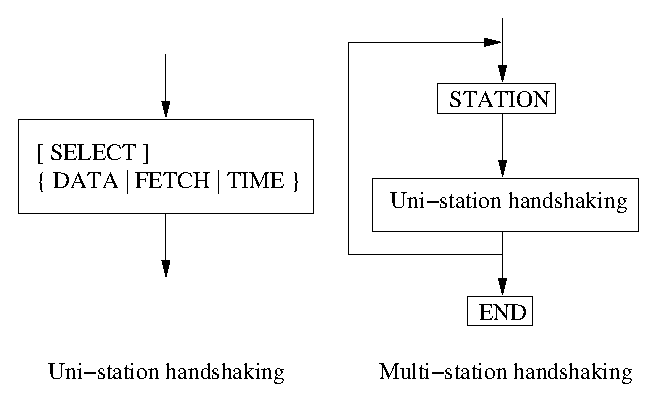
\includegraphics{handshaking.eps}
\caption{Handshaking in uni-station vs. multi-station mode} \label{handshaking}
\end{figure}


\subsection{Data Transfer}

When handshaking has been completed the server starts sending data
packets, each of which consists of an 8-byte SeedLink header followed
by a 512-byte Mini-SEED record. The SeedLink header is an ASCII string
consisting of the letters ``SL'' followed by a six-digit hexadecimal
packet sequence number. Each station has it own sequence numbers so if
multiple stations are requested using a single TCP channel the client
should look at the contents of Mini-SEED packet to determine the
station name (to maintain current sequence numbers for each
station). A sequence number in the same format is used as an argument
to ``DATA'' or ``FETCH'' command to start the data transfer from a
particular packet. Each SeedLink node re-assigns sequence numbers for
technical reasons, so it is not possible to use the same sequence
numbers when communicating with alternative servers.

Within particular node the sequence numbers of a single station are
consecutive and wrap around at FFFFFF. This can be used by the client
to detect ``sequence gaps'' (e.g., some data has been missed by the
client due to long network outage or software bug). However, if stream
selectors are used the sequence numbers are only guaranteed to be in
increasing order (with wrap) because some packets might be filtered
out by the server. In this case the first packet is not necessarily
the one requested, but the nearest packet (not older than requested)
that matches installed selectors.

The data is transferred as a continuous stream without any error
detections or flow control because these functions are performed by
the TCP protocol. This guarantees the highest data transfer rate that
is possible with the particular hardware and TCP/IP implementation.

Obviously, the average data transfer rate must be greater than the
rate at which new data becomes ready to send at the server. If this is
the case, sooner or later the server has sent all data available to
the client. When this happens, depending on the SeedLink mode, the
server sends new data as soon as it arrives or appends ASCII string
``END'' to the last packet and waits for the client to close
connection. The latter mode is called ``dial-up mode'' because it is
normally used in conjunction with dial-up lines to open the connection
periodically for a short time and download all data available. A
SeedLink packet can never start with ``END'' thus no ambiguity
arises.


\subsection{Commands} \label{commands}

\begin{interface}

\item HELLO

responds with a two-line message (both lines terminated with
CR+LF). The first line contains the version number of the SeedLink
daemon, the second line contains station or data center description
specified in the configuration. HELLO is used mainly for testing a
SeedLink server with ``telnet''.  It is also used by \verb+libslink+
to determine the server version.

\item CAT

shows the station list. Used mainly for testing a SeedLink server with
``telnet''.

\item BYE

closes the connection. Used mainly for testing a SeedLink server with
``telnet''.

\item STATION <station_code> <[network_code]>

turns on multi-station mode, used to transfer data of multiple
stations over a single TCP channel. The STATION command, followed by
SELECT (optional) and FETCH, DATA or TIME commands is repeated for
each station and the handshaking is finished with END.

STATION is a modifier command (it modifies the function of subsequent
SELECT, and DATA, FETCH or TIME commands) so it responds with ``OK'' on
success, ``ERROR'' otherwise.

\item END

end of handshaking in multi-station mode. This is an action command,
because it starts data transfer. No explicit response is sent.

\item SELECT <[pattern]>

when used without \<pattern>, cancels all selectors. Otherwise, if
\<pattern> is a positive selector, without leading ``!'', broadens the
selection of Mini-SEED streams; if \<pattern> is a negative selector,
with leading ``!'', narrows the selection of Mini-SEED streams. Only
one selector can be used in single \verb+SELECT+ request. A SeedLink
packet is sent to client if it matches any positive selector and
doesn't match any negative selectors.

General format of selectors is LLCCC.T where LL is location, CCC is
channel, and T is type (one of DECOTL for data, event, calibration,
blockette, timing, and log records). ``LL'', ``.T'', and ``LLCCC.'' can be
omitted, meaning ``any''. It is also possible to use ``?'' in place of L
and S.  Some examples can be found in table~\ref{selectors}.

\begin{table}[ht]
\centering
\begin{tabular}{|l|l|} \hline
Selectors used & Mini-SEED streams transferred               \\ \hline\hline
BH?            & BHZ, BHN, BHE (all record types)            \\ \hline
BH?.D          & BHZ, BHN, BHE (data records)                \\ \hline
00BH?.D        & BHZ, BHN, BHE with location code '00' (data records) \\ \hline
BH? !E         & BHZ, BHN, BHE (excluding detection records) \\ \hline
BH? E          & BHZ, BHN, BHE plus detection records of all \\
               & channels                                    \\ \hline
!LCQ !LEP      & all except LCQ and LEP channels             \\ \hline
!L !T          & all except log and timing records           \\ \hline
\end{tabular}
\caption{Selector examples} \label{selectors}
\end{table}

SELECT is a modifier command (it modifies the function of subsequent DATA,
FETCH or TIME commands) so it responds with ``OK'' on success, ``ERROR''
otherwise.

\item DATA <[n [begin_time]]>

in multi-station mode this sets the current station into real-time
mode and (optionally) the current sequence number to \<n>; in
uni-station mode this starts data transfer in real-time mode from
packet \<n> or from the next packet available if used without
arguments. If \<begin_time> is used, any older packets are filtered
out. \<begin_time> should be in the form of 6 decimal numbers
separated by commas in the form: year,month,day,hour,minute,second,
e.g. '2002,08,05,14,00'.

DATA is a modifier command in multi-station mode (responds with ``OK''
or ``ERROR''); in uni-station mode it is an action command (no
explicit response is sent).

\item FETCH <[n [begin_time]]>

works like DATA but sets the station to dial-up mode instead of
real-time mode.

\item TIME <[begin_time [end_time]]>

extracts time window from \<begin_time> to \<end_time>.  The times are
specified in the form of 6 decimal numbers separated by commas in the
form: year,month,day,hour,minute,second, e.g. '2002,08,05,14,00'.

\item INFO <level>

requests an INFO packet containing XML data embedded in a Mini-SEED
log record. \<level> should be one of the following: ID, CAPABILITIES,
STATIONS, STREAMS, GAPS, CONNECTIONS, ALL. The XML document conforms
to the DTD shown in section~\ref{infodtd}. The amount of info
available depends on the configuration of the SeedLink server.

\end{interface}


\section{Troubleshooting}

If SeisComP is not functioning correctly, it is recommended to first check
the log files in the ``logs'' directory, /var/log/messages and
/var/log/seedlink.  In order to find the error quickly, it is neccesary to
understand that the data goes through the following major components of the
system:
\begin{itemize}
\item plugin,
\item SeedLink's plugin interface,
\item SeedLink's StreamProcessor,
\item SeedLink's I/O system,
\item SeedLink's StreamMonitor,
\item clients (slarchive, etc.).
\end{itemize}

Often the malfunction of data acquisition is caused by generic operating
system errors such as disk corruption, therefore it is very important to
check /var/log/messages if the system behaves strangely.

In the following, we will take a look at errors that can happen in each of
the components.


\subsection{Plugin}

A plugin is just a normal program that sends data to file descriptor 63
(opened by SeedLink before it executes the plugin). Have a look at a
plugin definition in seedlink.ini; it is similar to the following:

\begin{verbatim}
plugin edata_EDD cmd="/home/sysop/bin/serial_plugin -v -f /home/sysop/config/plugins.ini"
             timeout = 600
             start_retry = 60
             shutdown_wait = 10
\end{verbatim}

Using the command line shown, you can run the plugin standalone as follows
(note that the plugin name is appended to the command line):

\begin{verbatim}
serial_plugin -v -f /home/sysop/config/plugins.ini edata_EDD 63>data.dat
\end{verbatim}

(before you do it, shut down the aquisition to make sure no other plugin
instances are running). Here we asked the shell to pre-open the file
descriptor 63 and re-direct it to file data.dat (this syntax does not work
with C-shell).

If the plugin works, then data (in SeedLink's internal format) should
appear in the file data.dat. Log messages are sent to standard output. If
no data arrives, check if baudrate and other settings are correct in
plugins.ini. It is usually possible to increase verbosity by -v flag or by
editing plugins.ini. Some plugins print a help message if -{}-help flag is
used.


\subsection{SeedLink's Plugin Interface}

In SeedLink, there is no one-to-one relation between stations and plugin
instances. For example, seismic channels and environmental (state of
health) channels can be digitized by different digitizers which are handled
by different plugins.

On the other hand, often a single plugin instance collects data of many
stations. This is the case with chain\_plugin, as well as other plugins
that connect to data acquisition systems.

Therefore each data packet sent by a plugin to file descriptor 63 contains
station ID, which tells SeedLink to which station this data belongs. If
SeedLink does not know this station, the data is ignored and a warning is
written to seedlink log file, which looks similar to the following%
\footnote{If ``dynamic\_stations=enabled'' is set in seedlink.ini, new
stations are added automatically, however, such stations are not supported
by the StreamProcessor, so only Mini-SEED data is accepted from a plugin.}:

\begin{verbatim}
Jun 26 03:47:22 st27 seedlink: [chain] station AMZI is not configured
\end{verbatim}


\subsection{SeedLink's StreamProcessor}

While Mini-SEED streams go straight to the I/O System, raw streams pass the
StreamProcessor module, which is probably the most problematic part of
SeedLink for inexperienced users.

The StreamProcessor is enabled by pointing the parameters ``streams'' and
``filters'' in seedlink.ini to respective configuration files. If
StreamProcessor is not enabled, then raw datastreams are ignored and you
can see warning in seedlink log file that looks like this:

\begin{verbatim}
Feb 19 13:24:23 st27 seedlink: KRIS raw data ignored
\end{verbatim}

The next possible error is mismatch between names or sample rates of raw
channels and stream processing scheme used. When you look at a station
definition in seedlink.ini, you can see something similar to the following:

\begin{verbatim}
station EDD  description = "GEOFON_Station"
             name = EDD
             network = GE
             proc = edata_100
\end{verbatim}

The ``proc'' attribute selects the stream processing scheme. If this
attribute is missing, raw data is not accepted and you will get the error
shown above.

The stream processing schemes are defined in the file streams.xml. The
scheme ``edata\_100'' is in fact based on two other schemes defined in this
file:

\begin{verbatim}
  <proc name="edata_100">
    <using proc="generic_6x100"/>
    <using proc="edata_aux"/>
  </proc>
\end{verbatim}

The scheme ``generic\_6x100'' is defined as follows:

\begin{verbatim}
  <proc name="generic_6x100">
    <tree>
      <input name="Z" channel="Z" location="" rate="100"/>
      <input name="N" channel="N" location="" rate="100"/>
      <input name="E" channel="E" location="" rate="100"/>
  
<!--  Uncomment this to enable 100Hz HH? streams  -->
<!--                                              -->
<!--  <node stream="HH"/>                         -->

<!--  Uncomment this to enable 50Hz SH? streams   -->
<!--                                              -->
<!--  <node filter="F96C" stream="SH"/>           -->

      <node filter="FS2D5" stream="BH">
        <node filter="F96C">
          <node filter="ULP" stream="LH">
            <node filter="VLP" stream="VH"/>
          </node> 
        </node>
      </node>
    </tree>
    <tree>
      <input name="Z1" channel="Z" location="" rate="100"/>
      <input name="N1" channel="N" location="" rate="100"/>
      <input name="E1" channel="E" location="" rate="100"/>

<!--  Uncomment this to enable 100Hz HN? streams  -->
<!--                                              -->
<!--  <node stream="HN"/>                         -->

      <node filter="F96C" stream="SN"/>
    </tree>
  </proc>
\end{verbatim}

This scheme tells the StreamProcessor how to create 12 streams (BHZ, BHN,
BHE, LHZ, LHN, LHE, VHZ, VNH, VHE, SNZ, SNN, SNE) from 6 raw input channels
(Z, N, E, Z1, N1, E1). Each raw data packet sent by a plugin is labeled
with channel ID in addition to station ID, so the StreamProcessor knows
which packet belongs to which channel.

Sometimes the channel ID's are hardcoded within a plugin, but often they
can be defined by a user. For example, in case of serial\_plugin the
following can be found in plugins.ini:

\begin{verbatim}
* Keyword 'channel' is used to map input channels to symbolic channel
* names. Channel names are arbitrary 1..10-letter identifiers which
* should match the input names of the stream processing scheme in
* stream.xml, which is referenced from seedlink.ini

channel Z source_id=0
channel E source_id=1
channel N source_id=2

* "State of health" channels

channel S0 source_id=16
channel S1 source_id=17
channel S2 source_id=18
channel S3 source_id=19
channel S4 source_id=20
channel S5 source_id=21
channel S6 source_id=22
channel S7 source_id=23
channel S8 source_id=24
\end{verbatim}

If a plugin uses channel ID, which is not defined in the stream processing
scheme, a warning similar to the following is shown:

\begin{verbatim}
Jun 24 12:56:28 st55 seedlink: EDD channel X ignored
\end{verbatim}

It is also important that the actual sample rate of raw channels is the
same as defined in the scheme, otherwise the time calculation is wrong and
there will be apparent gaps in data:

\begin{verbatim}
Jun 26 02:26:18 st27 seedlink: AMZI : Z time gap -8.15 seconds (detected)
\end{verbatim}


\subsection{SeedLink's I/O System}

If a plugin sends Mini-SEED data SeedLink, the StreamProcessor will not be
used and thus the SeedLink configuration will be much simpler. However,
still some problems may occur. First of all, the user must make sure that
the Mini-SEED data that comes from the plugin is correct big-endian
Mini-SEED---often there are errors in data because the authors of plugins
have not taken the differences between computer architectures into account
(eg., the Mini-SEED data is little-endian, which is not valid and not
supported by SeedLink).

Next source of problems is the corruption of SeedLink's disk buffer (files
in the directory pointed by the ``filebase'' parameter in seedlink.ini) due
to disk errors (bad blocks, etc.), which can cause strange error messages
and data gaps. In this case there are often disk errors shown in
/var/log/messages. If the SeedLink's disk buffer is corrupted, a simple fix
is to just delete its content.

Note that the SeedLink's disk buffer is only used by the SeedLink server
itself---modifying the buffer while SeedLink is running is not allowed.
When SeedLink is stopped, you can remove the buffer or use it for debugging
purposes (the files in buffer are in Mini-SEED format).


\subsection{SeedLink's StreamMonitor}

The module StreamMonitor is activated by setting the parameter
``stream\_check'' in seedlink.ini to ``enabled''. In this case the time
spans and gaps of streams are monitored (according to parameters
``gap\_check\_pattern'' and ``gap\_treshold'') and the information can be
requested from the server using \verb+slinktool+. The stream information is
also required for time window extraction.

When SeedLink exits, it saves the stream information of each station to a
file called buffer.xml, which is located in a subdirectory within the
SeedLink's disk buffer. In this case SeedLink can start fast, because it
can restore the stream information without scanning the disk buffer.
However, if the parameters ``stream\_check'', ``gap\_check\_pattern'' or
``gap\_treshold'' were meanwhile changed, the stored stream information may
not be valid. Therefore the buffer.xml files must be removed before
starting SeedLink. Scanning the disk buffer may take long time (depending
on its size and harddisk speed) and during that time it is not possible to
stop SeedLink (except with ``kill -9''). If you believe that scanning the
disk buffer is slower than it should be, check your operating system's IDE
DMA settings, however, fast DMA modes may also be less reliable.

When using the StreamMonitor, make sure that ``gap\_treshold'' is not too
low. In case of some digitizers, small gaps between records are normal due
to timing errors. Also, ``gap\_check\_pattern should be set such that
triggered streams are not included. Keeping track of a large number of gaps
may require more memory than available, causing a system crash.
 

\subsection{Clients}

If the SeedLink server seems to work correctly and data appears in the
SeedLink's disk buffer, but nothing is saved in the ``archive'' directory,
most probably the ``slarchive'' client is not running properly.

The clients acquire data from the SeedLink server only via TCP/IP, even if
they are running on the local machine. When a client starts, the SeedLink
commands it sends are listed in the SeedLink log file. Using
\verb+slinktool+, you can check which clients are connected, what is the
status of connections (eg., if there are many packets in the Queue, the
client may be hanging or there may be network errors that prevent it from
getting data). If the StreamMonitor is enabled, \verb+slinktool+ can also
show the timespans of streams in the buffer.

You can also telnet to the SeedLink server and use the commands listed in
section~\ref{commands} directly:

\begin{verbatim}
$ telnet localhost 18000
Trying 139.17.3.25...
Connected to geofon.gfz-potsdam.de.
Escape character is '^]'.
HELLO
SeedLink v3.0 (2004.129)
GEOFON DC
BYE
Connection closed by foreign host.
\end{verbatim}

Network connections can be also tested with \verb+slinktool+. The following
command will request station APE from the GEOFON server and print verbose
information about every packet received:

\begin{verbatim}
slinktool -vvv -S GE_APE geofon.gfz-potsdam.de:18000
\end{verbatim}


\clearpage

%%%%%%%%%%%%%%%%%%%%%%%%%%%%%%% Appendices %%%%%%%%%%%%%%%%%%%%%%%%%%%%%%%%

\newcommand{\CodeFile}[1]{%
    \subsection{#1}\leavevmode
    \normalfont\ttfamily\scriptsize
    \verbinput{#1}}

\appendix

\section{SeisComP Data Structure (SDS) definition}\label{sds}
\normalfont\ttfamily\scriptsize
\verbinput{SDS.definition}

\section{XML DTDs}\label{dtds}
\CodeFile{streams.dtd}
\CodeFile{seedlink.dtd}\label{infodtd}
\CodeFile{chain.dtd}

\end{document}

